\chapter{L�sungen}
\section{Mengen}
\subsection{Sportverein}
\label{sec:Loesung-Mengen-Sportverein}
L�sung zu Aufgabe \vref{sec:Aufgabe-Mengen-Sportverein}.

\begin{description}
	\item[$H$] ist die Menge aller Handballspieler
	\item[$F$] ist die Menge aller Fu�ballspieler
	\item[$E$] ist die Menge aller Eisl�ufer
	\item[$S$] ist die Menge aller Skifahrer
	\item[$V$] ist die Menge aller Vereinsmitglieder
\end{description}

Durch die Aufgabenstellung gilt das folgende:
\begin{itemize}
	\item $\emptyset=H\cap F$
	\item $E\subseteq F$
	\item $E\cup S=V$
\end{itemize}

Es gilt die Behauptung:\\
\qquad$H\subseteq S$

Es folgt der Beweis:
\begin{alignat*}{2}
&H = H\cap V &&=\\
&H\cap(E\cup S) &&=\\
&(H\cap E)\cup(H\cap S)\subseteq(H\cap F)\cup(H\cap S) &&=\\
&\emptyset\cup(H\cap S) &&=\\
&H\cap S\subseteq S
&\end{alignat*}

\subsection{Aufgabe 1}
\label{sec:Loesung-Mengen-AufgabeEins}
L�sung zu Aufgabe \vref{sec:Aufgabe-Mengen-AufgabeEins}.

\begin{enumerate}
\item TODO
\item TODO
\end{enumerate}

\subsection{Aufgabe 2}
\label{sec:Loesung-Mengen-AufgabeZwei}
L�sung zu Aufgabe \vref{sec:Aufgabe-Mengen-AufgabeZwei}.

\begin{multicols}{3}
\begin{enumerate}
	\item TODO
	\item TODO
	\item TODO
	\item TODO
	\item TODO
	\item TODO
\end{enumerate}
\end{multicols}
\renewcommand{\labelenumi}{\arabic{enumi}.}

\section{Logik}
\subsection{Aufgabe 1.2}
\label{sec:Loesung-Logik-AufgabeEinsPunktZwei}
L�sung zu Aufgabe \vref{sec:Aufgabe-Logik-AufgabeEinsPunktZwei}.

\begin{multicols}{3}
\renewcommand{\labelenumi}{zu \alph{enumi})}
\begin{enumerate}
\item $ $ \newline
		%TABL-09.10.2008-mathe-1
		\begin{tabular}{c|c||c}
		$A$ & $B$ & \\
		\hline
		$w$ & $w$ & $f$\\
		$w$ & $f$ & $f$\\
		$f$ & $w$ & $w$\\
		$f$ & $f$ & $f$\\
		\end{tabular}

\item $ $ \newline
		%TABL-09.10.2008-mathe-2
		\begin{tabular}{c|c||c}
		$A$ & $B$ & \\
		\hline
		$w$ & $w$ & $w$\\
		$w$ & $f$ & $f$\\
		$f$ & $w$ & $w$\\
		$f$ & $f$ & $w$\\
		\end{tabular}

\item $ $ \newline
		%TABL-09.10.2008-mathe-3
		\begin{tabular}{c|c||c}
		$A$ & $B$ & \\
		\hline
		$w$ & $w$ & $f$\\
		$w$ & $f$ & $w$\\
		$f$ & $w$ & $f$\\
		$f$ & $f$ & $f$\\
		\end{tabular}
\end{enumerate}
\end{multicols}

\subsection{Aufgabe 1.3}
\label{sec:Loesung-Logik-AufgabeEinsPunktDrei}
L�sung zu Aufgabe \vref{sec:Aufgabe-Logik-AufgabeEinsPunktDrei}.

\renewcommand{\labelenumi}{zu \alph{enumi})}
\begin{enumerate}
\item $A = 18$ ist durch $12$ teilbar\\
		$B = 18$ ist durch $3$ teilbar\\
		$A$ falsch, $B$ richtig $\Ra$ $A \Rightarrow B$ wahr
\item $A = 3$ ist Teiler von $8$\\
		$B = 14$ ist eine Primzahl\\
		$A$ falsch, $B$ falsch $\Ra$ $A \Leftrightarrow B$ wahr
\end{enumerate}
\renewcommand{\labelenumi}{\arabic{enumi}.}

\subsection{Aufgabe 6}
\label{sec:Loesung-Logik-AufgabeSechs}
L�sung zu Aufgabe \vref{sec:Aufgabe-Logik-AufgabeSechs}.

\renewcommand{\labelenumi}{zu \alph{enumi})}
\begin{enumerate}
\item $ $ \newline
		\begin{tabular}{c|c||c|c|c}
		$A$ & $B$ & $(\neg (A \und B))$ & $((\neg A) \oder B)$ & $(\neg (A \und B)) \und ((\neg A) \oder B)$
		\\\hline
		$w$ & $w$ & $f$ & $w$ & $f$
		\\$w$ & $f$ & $w$ & $f$ & $f$
		\\$f$ & $w$ & $w$ & $w$ & $w$
		\\$f$ & $f$ & $w$ & $w$ & $w$
		\end{tabular}
\item $ $ \newline
		\begin{tabular}{c|c||c}
		$A$ & $B$ & $((\neg A) \oder B) \Ra (A \und B)$
		\\\hline
		$w$ & $w$ & $w$
		\\$w$ & $f$ & $w$
		\\$f$ & $w$ & $f$
		\\$f$ & $f$ & $f$
		\end{tabular}
\end{enumerate}
\renewcommand{\labelenumi}{\arabic{enumi}.}

\subsection{Aufgabe 7}
\label{sec:Loesung-Logik-AufgabeSieben}
L�sung zu Aufgabe \vref{sec:Aufgabe-Logik-AufgabeSieben}.

\renewcommand{\labelenumi}{zu \alph{enumi})}
\begin{enumerate}
\item $ $ \newline
		\begin{tabular}{c|c|c||c|c|c}
		$A$ & $B$ & $C$ & $(A \oder B)$ & $\neg C$ & $(A \oder B) \Ra \neg C$
		\\\hline
		$w$ & $w$ & $w$ & $w$ & $f$ & $f$
		\\$w$ & $w$ & $f$ & $w$ & $w$ & $w$
		\\$w$ & $f$ & $w$ & $w$ & $f$ & $f$
		\\$w$ & $f$ & $f$ & $w$ & $w$ & $w$
		\\$f$ & $w$ & $w$ & $w$ & $f$ & $f$
		\\$f$ & $w$ & $f$ & $w$ & $w$ & $w$
		\\$f$ & $f$ & $w$ & $f$ & $f$ & $w$
		\\$f$ & $f$ & $f$ & $f$ & $w$ & $w$
		\end{tabular}
\item $ $ \newline
		\begin{tabular}{c|c|c||c|c|c}
		$A$ & $B$ & $C$ & $\neg A$ & $\neg B$ & $C \Ra (\neg A) \und (\neg B)$
		\\\hline
		$w$ & $w$ & $w$  & $f$ & $f$ & $w$  
		\\$w$ & $w$ & $f$ & $f$ & $f$ & $w$
		\\$w$ & $f$ & $w$ & $f$ & $w$ & $w$
		\\$w$ & $f$ & $f$ & $f$ & $w$ & $w$
		\\$f$ & $w$ & $w$ & $w$ & $f$ & $w$
		\\$f$ & $w$ & $f$ & $w$ & $f$ & $w$
		\\$f$ & $f$ & $w$ & $w$ & $w$ & $w$
		\\$f$ & $f$ & $f$ & $w$ & $w$ & $w$
		\end{tabular}
\end{enumerate}
\renewcommand{\labelenumi}{\arabic{enumi}.}

\subsection{Aufgabe 8}
\label{sec:Loesung-Logik-AufgabeAcht}
L�sung zu Aufgabe \vref{sec:Aufgabe-Logik-AufgabeAcht}.

$\begin{array}{rcl}
	F_1 &=& \neg A \und B\\
	F_2 &=& \neg B \und A\\
	F_3 &=& (\neg F_1) \und (\neg F_2)\\
	&=& (\neg(\neg A \und B)) \und (\neg(\neg B \und A))\\
	&=& (\neg(\neg A) \oder \neg B) \und (\neg(\neg B) \oder \neg A)\\
	&=& (A \oder \neg B) \und (B \oder \neg A)\\
	&=& (A \und B) \oder \neg (A \oder B)\\
	&=& (A \und B) \oder (\neg A \neg B)
\end{array}$

\subsection{Aufgabe 9}
\label{sec:Loesung-Logik-AufgabeNeun}
L�sung zu Aufgabe \vref{sec:Aufgabe-Logik-AufgabeNeun}

\subsubsection{Aufgaben L�sung}
\begin{tabular}{c|c|c|c||c|c|c}
$A$ & $B$ & $C$ & $D$ & $(A \oder B) \und D$ & $\overline{(A \oder B)} \und (C \oder D)$ & $C \Ra ((A \und D) \oder (B \und D))$
\\\hline
$f$ & $w$ & $f$ & $w$ & $w$ & $f$ & $w$\\
$w$ & $w$ & $w$ & $f$ & $f$ & $f$ & $f$\\
$f$ & $f$ & $f$ & $w$ & $f$ & $w$ & $w$
\end{tabular}

\subsection{Aufgabe 9}
\label{sec:Loesung-Logik-AufgabeZehn}
L�sung zu Aufgabe \vref{sec:Aufgabe-Logik-AufgabeZehn}

\renewcommand{\labelenumi}{zu \alph{enumi})}
\begin{enumerate}
\item $\forall x \in \mathbb{N}: x^2$ gerade\\
		$\neg (A x \in \mathbb{N}_0: x^2$ gerade\\
		$\aeq \exists x \in \mathbb{N}_0: x^2$ nicht gerade\\
		Es gibt mindestens eine ungerade Quadratzahl
\item $\exists n \in \mathbb{N}: n \notin \mathbb{Q}$\\
		$\neg (\exists n \in \mathbb{N}: n \notin \mathbb{Q})$\\
		$\aeq \forall n \in \mathbb{N}: n \in \mathbb{Q}$
\item $\neg((\forall$ Stra�en f�hren nach Rom) $\und$ ($\exists$ Pfad f�hrt nach Rom))\\
		$\aeq(\neq(\forall$ Stra�en f�hren nach Rom)) $\oder$ $(\neq (\exists$ Pfad f�hrt nach Rom))\\
		$\aeq(\exists$ Stra�e, die nicht nach Rom f�hrt) $\oder$ $(\forall$ Pfade f�hren nicht nach Rom)
\end{enumerate}
\renewcommand{\labelenumi}{\arabic{enumi}.}

\section{Relationen und Abbildungen}
\subsection{Aufgabe 1.4}
\label{sec:Loesung-RelationenUndAbbildungen-EinsPunktVier}
L�sung zu Aufgabe \vref{sec:Aufgabe-RelationenUndAbbildungen-EinsPunktVier}

\renewcommand{\labelenumi}{zu \alph{enumi})}
\begin{enumerate}
\item $R = $\gklamm{(1,1), (1,2), (1,3), (1,4), (3,1), (3,2), (3,3), (3,4)}
\item %TAB-15.10.2008-mathe-4
		\begin{minipage}{\textwidth}
		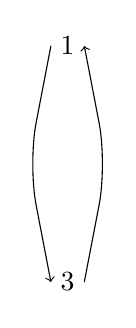
\begin{tikzpicture}
		%Nodes
		\node (Oben) 	at (0,0) 		{$1$};
		\node (Unten) 		at (0,-3) 		{$3$};

		%Verkn�pfungen
		\draw[->,rounded corners = 15pt] (Oben.west) -- (-0.5,-1.5) -- (Unten.west);
		\draw[->,rounded corners = 15pt] (Unten.east) -- (0.5,-1.5) -- (Oben.east);
		\end{tikzpicture}
		\end{minipage}
\item $\left(\begin{array}{cccc}
				 w & w & w & w\\
				 f & f & f & f\\
				 w & w & w & w\\
				 f & f & f & f
				 \end{array}\ \right)$
\end{enumerate}
\renewcommand{\labelenumi}{\arabic{enumi}.}

\subsection{Aufgabe 1.5}
\label{sec:Loesung-RelationenUndAbbildungen-EinsPunktFuenf}
L�sung zu Aufgabe \vref{sec:Aufgabe-RelationenUndAbbildungen-EinsPunktFuenf}

\begin{tabular}{r|c|c|c}
				& a 	& b 	& c\\
\hline
reflexiv		& x 	& 	& \\
\hline
symmetrisch	& x	& 	& \\
\hline
transitiv	& x 	& x	& x\\
\end{tabular}
\renewcommand{\labelenumi}{\arabic{enumi}.}

\section{Matrizen und Determinanten}
\subsection{Aufgabe 3.3}
\label{sec:Loesung-MatrizenundDeterminanten-Aufgabe-3-3}
L�sung zu Aufgabe \vref{sec:Aufgabe-MatrizenundDeterminanten-Aufgabe-3-3}
\begin{enumerate}
\item $A \mal B$
		\[= \varvektor{cc}{2 & -1\\1 & 0\\-3 & 4} \mal \varvektor{ccc}{1 & -2 & -5\\3 & 4 & 0} \in M(3, 3)\]
		\[= \varvektor{ccc}{2 - 3 & -4 - 4 & -10 + 0\\1 + 0 & -2 + 0 & -5 + 0\\-3 + 12 & 6 + 15 & 15 + 0} = \varvektor{ccc}{-1 & -8 & -10\\1 & -2 &-5\\9 & 22 & 15}\]

\item $B \mal A$
		\[= \varvektor{ccc}{1 & -2 & -5\\3 & 4 & 0} \mal \varvektor{cc}{2 & -1\\1 & 0\\-3 & 4} \in M(2, 2)\]
		\[= \varvektor{cc}{2 - 2 + 15 & -1 + 0 -20\\6 + 4 + 0 & -3 + 0 + 0} = \varvektor{cc}{15 & -21\\10 & -3}\]

\item $C \mal D$
		\[= \varvektor{cc}{1 & 6\\-3 & 5} \mal \varvektor{cc}{4 & 0\\2 & -1} = \varvektor{cc}{4 + 12 & 0 - 6\\-12 + 10 & 0 - 5} = \varvektor{cc}{16 & -6\\-2 & -5}\]

\item $D \mal C$
		\[= \varvektor{cc}{4 & 0\\2 & -1} \mal \varvektor{cc}{1 & 6\\-3 & 5} = \varvektor{cc}{4 + 0 & 24 + 0\\2 + 3 & 12 - 5} = \varvektor{cc}{4 & 24\\5 & 7}\]
\end{enumerate}

\section{Vollst�ndige Induktion}
\subsection{Aufgabe A16}
\label{sec:Loesung-VollstaendigeInduktion-A16}
L�sung zu Aufgabe \vref{sec:Aufgabe-VollstaendigeInduktion-A16}

Induktionsschluss von $n = 1$ auf $n +1 = 2$ ist falsch, denn die beiden einelementigen Teilmengen haben keine Schnittmenge $\neq \emptyset$.

\section{Vektorraum}
\subsection{Aufgabe 4.5}
\label{sec:Loesung-Vektorraum-A4.5}
L�sung zu Aufgabe \vref{sec:Aufgabe-Vektorraum-A4.5}
\[A^2 = \varvektor{rrr}{4 & -6 & 6\\3 & -5 & 6\\3 & -6 & 7}\]
\[B = \gklamm{\varvektor{ccc}{1 & 0 & 0\\0 & 0 & 0\\0 & 0 & 0}, \varvektor{ccc}{0 & 1 & 0\\0 & 0 & 0\\0 & 0 & 0}, \dots, \varvektor{ccc}{0 & 0 & 0\\0 & 0 & 0\\0 & 1 & 0}, \varvektor{ccc}{0 & 0 & 0\\0 & 0 & 0\\0 & 0 & 1}}\]
\[(A)_B = \varvektor{c}{2\\-6\\6\\3\\-7\\6\\3\\-6\\5}, (A^2)_B = \varvektor{c}{4\\-6\\6\\3\\-5\\6\\3\\-6\\7}, (E_3)_B = \varvektor{c}{1\\0\\0\\0\\1\\0\\0\\0\\1}\]
\[\gauss{ccc|c}{2 & 4 & 1 & 0\\\vdots & \vdots & \vdots & \vdots\\5 & 7 & 1 & 0} \ra \gauss{ccc|c}{2 & 4 & 1 & 0\\3 & 3 & 0 & 0\\-7 & 5 & 1 & 0\\5 & 7 & 1 & 0} \ra \gauss{ccc|c}{2 & 4 & 1 & 0\\3 & 3 & 0 & 0}\]
\[\ra \gauss{ccc|c}{2 & 4 & 1 & 0\\0 & -3 & 1 \frac{1}{2} & 0}\]
$\Ra$ $A$, $A^2$, $E_3$ sind linear abh�ngig

\subsection{Aufgabe 4.7}
\label{sec:Loesung-Vektorraum-A4.7}
L�sung zu Aufgabe \vref{sec:Aufgabe-Vektorraum-A4.7}
\begin{align*}
	\varvektor{rr}{1 & -2\\3 & 4} &= x_1 \varvektor{cc}{0 & 1\\1 & 0} + x_2 \varvektor{cc}{0 & -1\\0 & 0} + x_3 \varvektor{cc}{1 & -1\\0 & 3} + x_4 \varvektor{cc}{0 & 1\\0 & 1}\\
	&\Leftrightarrow \varvektor{c}{1\\-2\\3\\4} = x_1 \varvektor{c}{0\\1\\1\\0} + x_2 \varvektor{c}{0\\-1\\0\\0} + x_3 \varvektor{c}{1\\-1\\0\\3} + x_4 \varvektor{c}{0\\1\\0\\1}\\
	&\Leftrightarrow \gauss{rrrr|r}{0 & 0 & 1 & 0 & 1\\1 & -1 & -1 & 1 & -2\\1 & 0 & 0 & 0 & 3\\0 & 0 & 3 & 1 & 4} \underrightarrow{\RM{1} \leftrightarrow \RM{3}}\\
	&\underrightarrow{\RM{2} = \RM{2} (-1)}_{\RM{4} = \RM{4} - 3 \RM{2}}\\
	&\underrightarrow{\RM{2} = \RM{2} + \RM{4}}\\
	&\underrightarrow{\RM{2} = \RM{2} - \RM{3}}\\
	\varvektor{rr}{1 & -2\\3 & 4}_{\mathcal{B}} = \varvektor{c}{3\\5\\1\\1}
\end{align*}

\subsection{Aufgabe 4.8}
\label{sec:Loesung-Vektorraum-A4.8}
L�sung zu Aufgabe \vref{sec:Aufgabe-Vektorraum-A4.8}
\begin{enumerate}[label=\alph*)]
\item $\vektor{3}{-5}{4} = x_1 \vektor{1}{0}{0} + x_2 \vektor{1}{1}{0} + x_3 \vektor{1}{1}{1}$\\
		$\gauss{ccc|c}{1 & 1 & 1 & 3\\0 & 1 & 1 & -5\\0 & 0 & 1 & 4} \underrightarrow{\RM{1} = \RM{1} - \RM{2}}$\\
		$\underrightarrow{\RM{2} = \RM{2} - \RM{3}}$\\
		$\Ra \vec{U}_{\mathcal{B}} = \vektor{8}{-9}{4}$

\item $\vec{v} = -4 \mal \vektor{1}{0}{0} + 8 \vektor{1}{1}{0} - 7 \vektor{1}{1}{1} = \vektor{-4 + 8 - 7}{0 + 8 - 7}{0 + 0 - 7} = \vektor{-3}{1}{-7}$
\end{enumerate}

\section{Euklidischer Vektorraum $\mathbb{R}^n$}
\subsection{Aufgabe 5.1}
\label{sec:Loesung-EukVektorraum-A5.1}
L�sung zu Aufgabe \vref{sec:Aufgabe-EukVektorraum-A5.1}
\[\vec{v} = \vektor{a}{b}{c}, \vec{u} = \vektor{-1}{2}{3}\]
\[\vec{v} \mal \vec{u} = -a + 2b + 3c = 0\]
\begin{align*}
	F &= \gklamm{\vektor{a}{b}{c} \in \mathbb{R}^3 \vert -a + 2b + 3c = 0, a, b, c \in \mathbb{R}}\\
	&= \gklamm{\underbrace{\vektor{2b + 3c}{b}{c}}_{b \mal \vektor{2}{1}{0} + c \mal \vektor{3}{0}{1}} \in \mathbb{R}^3 \vert b, c \in \mathbb{R}}
\end{align*}
\subsection{Aufgabe 5.2}
\label{sec:Loesung-EukVektorraum-A5.2}
L�sung zu Aufgabe \vref{sec:Aufgabe-EukVektorraum-A5.2}
\[\vec{AB} = -(\vec{b} - \vec{a}) = \vektor{-(7 - 3)}{-(0 - (-2))}{-(11 - 12)} = \vektor{-4}{-2}{1}\]
\[\vec{AC} = -(\vec{c} - \vec{a}) = \vektor{-3}{5}{-2}\]
\[\vec{AB} \mal \vec{AC} = \alpha\]
\[\vec{AB} \mal \vec{AC} = 12 - 10 - 2 = 0 \Ra \alpha = 90�\]
